\RequirePackage[l2tabu,orthodox]{nag}  % warn about common LaTeX pitfalls
\RequirePackage[ascii]{inputenc}  % input is 7-bit ASCII
\RequirePackage{fixltx2e}  % fix LaTeX2e kernel bugs

\documentclass[11pt,twoside]{article}
\usepackage{color}
\usepackage{graphicx}
\graphicspath{ {image/} }
\usepackage{calc}  % arithmetic in length parameters
\usepackage{enumitem}  % more control over list formatting
\usepackage{fancyhdr}  % simpler headers and footers
\usepackage[margin=1in]{geometry}  % page layout
\usepackage{lastpage}  % for last page number
\usepackage{relsize}  % easier font size changes
\usepackage[normalem]{ulem}  % smarter underlining
\usepackage{url}  % verb-like typesetting of URLs
\usepackage{xfrac}  % nicer looking simple fractions for text and math
\usepackage{longtable}
\usepackage{tikz}
\usepackage{array}
\usepackage{tikz-timing}
\usetikzlibrary{arrows, shapes, backgrounds,fit}
\usepackage{tkz-graph}
% Set up fonts.
\usepackage[T1]{fontenc}  % use true 8-bit fonts
\usepackage{slantsc}  % allow slanted small-caps
\usepackage{microtype}  % perform various font optimizations
% Use Palatino-based monospace instead of kpfonts' default.
%\usepackage{newpxtext}
\ttfamily
\DeclareFontShape{T1}{\ttdefault}{m}{scsl}{<->ssub*\ttdefault/m/sc}{}
\DeclareFontShape{T1}{\ttdefault}{b}{scsl}{<->ssub*\ttdefault/b/sc}{}
% "Kepler" fonts.
\usepackage[nott,notextcomp]{kpfonts}
% Use curvier Latin Modern brackets instead of kpfonts' glyphs.
\DeclareSymbolFont{lmsymb}     {OMS}{lmsy}{m}{n}
\DeclareSymbolFont{lmlargesymb}{OMX}{lmex}{m}{n}
\DeclareMathDelimiter{\rbrace}{\mathclose}{lmsymb}{"67}{lmlargesymb}{"09}
\DeclareMathDelimiter{\lbrace}{\mathopen}{lmsymb}{"66}{lmlargesymb}{"08}

% Page layout: stretch text to fill up page.
\addtolength\footskip{.25\headheight}
\flushbottom

% Common list settings.

% Common macros.
%%  Common macros for the course CSC263H1 at the University of Toronto.
%%
%%  Copyright (c) 2014 Francois Pitt <fpitt@cs.utoronto.ca>
%%  last updated at 17:53 (EDT) on Sun 19 Oct 2014
%%
%%  CC BY-SA 4.0
%%  This work (the current file named 'macros-263.tex') is licensed under
%%  the Creative Commons Attribution-ShareAlike 4.0 International License.
%%  To view a copy of this license, visit
%%      http://creativecommons.org/licenses/by-sa/4.0/
%%  or send a letter to: Creative Commons, 444 Castro Street, Suite 900,
%%  Mountain View, California, 94041, USA.
%%  This is a human-readable summary of (and not a substitute for) the
%%  license.
%%  You are free to:
%%      Share -- copy and redistribute the material in any medium or format
%%      Adapt -- remix, transform, and build upon the material for any
%%          purpose, even commercially.
%%      The licensor cannot revoke these freedoms as long as you follow the
%%          license terms.
%%  Under the following terms:
%%      Attribution -- You must give appropriate credit, provide a link to
%%          the license, and indicate if changes were made. You may do so in
%%          any reasonable manner, but not in any way that suggests the
%%          licensor endorses you or your use.
%%      ShareAlike -- If you remix, transform, or build upon the material,
%%          you must distribute your contributions under the same license as
%%          the original.
%%      No additional restrictions -- You may not apply legal terms or
%%          technological measures that legally restrict others from doing
%%          anything the license permits.
%%  Notices:
%%      You do not have to comply with the license for elements of the
%%      material in the public domain or where your use is permitted by an
%%      applicable exception or limitation.
%%      No warranties are given. The license may not give you all of the
%%      permissions necessary for your intended use. For example, other
%%      rights such as publicity, privacy, or moral rights may limit how you
%%      use the material.

% Redefine \today in the style "DD Month YYYY".
\renewcommand*\today
 {\number\day\space\ifcase\month\or January\or February\or March\or
  April\or May\or June\or July\or August\or September\or October\or
  November\or December\fi\space\number\year}

% TeX trick so that math symbols are bold when text is.
\let\seiresfb\bfseries\def\bfseries{\boldmath\seiresfb}
\let\seiresdm\mdseries\def\mdseries{\unboldmath\seiresdm}

% Centered version of \llap and \rlap.
\providecommand*\clap[1]{\hbox to 0pt{\hss#1\hss}}

% Spacing macros with default argument.
\providecommand*\vfillstretch[1][1]{\vspace*{\stretch{#1}}}
\providecommand*\hfillstretch[1][1]{\hspace*{\stretch{#1}}}

% Abbreviations of latin phrases.
\let\latinabb\empty  % no special formatting
\providecommand*\ie{\latinabb{i.e.}}
\providecommand*\eg{\latinabb{e.g.}}
\providecommand*\etc{\latinabb{etc}}
\providecommand*\vs{\latinabb{vs}}

% General fonts and characters.
\let\longemph\textsl  % alternate way to emphasize
\let\strong\textbf  % strong emphasis
\let\code\texttt  % code fragments
\let\var\textsl  % multi-letter variables
\let\pred\mathbf  % predicates
\providecommand*\stup{\textsuperscript{st}}
\providecommand*\ndup{\textsuperscript{nd}}
\providecommand*\rdup{\textsuperscript{rd}}
\providecommand*\thup{\textsuperscript{th}}
\newcommand*\bbmath[1]{\ensuremath{\mathbb{#1}}}  % requires amssymb
\providecommand*\N{\bbmath{N}}  % requires amssymb
\providecommand*\Z{\bbmath{Z}}  % requires amssymb
\providecommand*\Q{\bbmath{Q}}  % requires amssymb
\providecommand*\R{\bbmath{R}}  % requires amssymb
\providecommand*\bigOh{\mathcal{O}}
\providecommand*\onehalf{\ensuremath{{}^1\!\!/\!_2}}
\providecommand*\letlinebreak{\penalty\exhyphenpenalty}
\providecommand*\halfthinspace{\kern.083333em}
\providecommand*\dash
   {\letlinebreak\halfthinspace---\halfthinspace\letlinebreak}
\let\per\slash  % for convenience

% For defined terms -- requires package ulem.
\newcommand*\defn[1]{\uline{\textit{#1}}}
\setlength{\ULdepth}{.2ex}

% General math macros.
\newcommand*\hiderel[1]{\mathrel{\hphantom{#1}}}
\providecommand*\comp[1]{\overline{#1}}  % set complement
\providecommand*\emptystr{\varepsilon}  % empty string
\providecommand*\lxor{\mathbin\oplus}  % exclusive or
\providecommand*\cat{\cdot}  % string concatenation
% Floors and ceilings, with optional size-changing command, e.g.,
% \floor[\Big]{x/2} becomes '\Big\lfloor{x/2}\Big\rfloor'.
\providecommand*\floor[2][]{{#1\lfloor}{#2}{#1\rfloor}}
\providecommand*\ceil[2][]{{#1\lceil}{#2}{#1\rceil}}
\providecommand*\lcm{\operatorname{lcm}}  % requires amsmath
\providecommand*\size{\operatorname{size}}  % requires amsmath
\providecommand*\len{\operatorname{len}}  % requires amsmath
\providecommand*\divides{\mathrel{|}}

% Redefined symbols from amssymb.
\renewcommand*\emptyset{\varnothing}  % rounder than default
\let\bigiff\iff
\renewcommand*\iff{\mathrel{\Leftrightarrow}}  % smaller than default
\let\bigimplies\implies
\renewcommand*\implies{\mathrel{\Rightarrow}}  % smaller than default
\renewcommand*\ge{\geqslant}  % with slanted line under the > sign
\renewcommand*\le{\leqslant}  % with slanted line under the < sign

% For algorithms, using either CLRS-style or Python-style pseudocode.
\let\ADT\textsc  % ADT names
\let\proc\textsc  % function names
\let\const\textsc  % constants (True, False, etc.)
\let\kw\textbf  % keywords (if, while, etc.)
\providecommand*\comm[1]{\textsl{\#\space#1}}  % comments
\providecommand*\opgets[1]{\mathrel{#1=}}
\providecommand*\eq{\mathrel{==}}
\providecommand*\True{\const{True}}
\providecommand*\False{\const{False}}
\providecommand*\None{\const{None}}
\providecommand*\cmod{\mathbin{\%}}
\providecommand*\nil{\const{nil}}

% Checkboxes and checklists.
% \checkmark already defined in amssymb
\makeatletter
\@ifpackageloaded{kpfonts}
   {\newcommand*\exmark{$\times$}}
   {\newcommand*\exmark{{\boldmath$\times$}}}
\makeatother
\newlength\exmarksize
\newlength\exmarkdepth
\newcommand*\checkbox[1][]
   {\settoheight\exmarksize{\exmark}
    \settodepth\exmarkdepth{\exmark}
    \addtolength\exmarksize{-\exmarkdepth}
    {\setlength\fboxrule{.1ex}\setlength\fboxsep{.1ex}%
    \fbox{\rule{0pt}{\exmarksize}\makebox[\exmarksize]{\smash{#1}}}}}
\newcommand*\checkedbox{\checkbox[\raisebox{.1ex}{\kern.2em$\checkmark$}]}
\newcommand*\exedbox{\checkbox[\exmark]}
\newenvironment*{checklist}{\begin{list}{\checkbox}{}}{\end{list}}
\newcommand*\checkeditem{\item[\checkedbox]}
\newcommand*\exeditem{\item[\exedbox]}
\newcommand*\boxeditem[1][]{\item[{\checkbox[#1]}]}

% Macros for drawing "underline" rules and half-boxes.
\providecommand*\urule[2][.5pt]{\rule[-.4ex]{#2}{#1}} % "underline" rule
% Underlined text box (with optional positioning argument).
\providecommand*\ubox[3][c]{\rlap{\urule{#2}}\makebox[#2][#1]{#3}}
% Underlined text box with caption (and optional caption positioning).
\providecommand*\capbox[5][c]{\ifx\empty#2\empty
    \else\rlap{\raisebox{-\baselineskip}{\makebox[#3][#1]{#2}}}\fi
    \ubox[#4]{#3}{#5}}

% For student numbers.
\providecommand*\hb{\urule{1.2em}}      % horizontal bar
\providecommand*\vb{\urule[1ex]{.5pt}}  % vertical bar
\providecommand*\studentnumberboxes     % now 10-digits long!
   {\vb\hb\vb\hb\vb\hb\vb\hb\vb\hb\vb\hb\vb\hb\vb\hb\vb\hb\vb\hb\vb}
\newlength\numberboxwidth
\settowidth\numberboxwidth{\studentnumberboxes}

% Command to format sample solutions for tutorials.
\newcommand\samplesolution[1]
   {\ifsolutions\begin{quote}\sffamily{#1}\end{quote}\fi}

% Marking-related macros.
\providecommand*\markitem[2][]
   {\item{\bfseries#2}\ifx\empty#1\empty\else
    \space[$#1$ mark\ifnum#1>1 s\fi]\fi:\quad\ignorespaces}
\providecommand*\errorcode[2][]
   {\item{\bfseries error code #2}\ifx\empty#1\empty\else
    \space[#1]\fi:\quad\ignorespaces}
\providecommand*\commonerror[1][]
   {\item{\bfseries common error}\ifx\empty#1\empty\else
    \space[#1]\fi:\quad\ignorespaces}
\makeatletter
\providecommand*\heading[1]%
   {\@startsection{heading}{9}{0pt}{-.75ex plus -1.5ex minus -.5ex}
    {-.5em plus -.5em minus -.25em}{\normalfont}*{\textsc{#1}}\mbox{}}
\makeatother
\newcommand*\st{\mathrel{|}}  % "such that" for set extension

% Headings.
\pagestyle{fancy}
\let\headrule\empty
\let\footrule\empty
\lhead{CSC\,336\,H1}
\chead{\large\scshape Assignment \#\,4}
\rhead{\scshape Fall 2015}
\lfoot{\scshape Dept.\@ of Computer Science, University of Toronto,
       St.~George Campus}
\cfoot{}
\rfoot{\scshape page \thepage\space of \pageref{LastPage}}


\begin{document}
\center Rui Ji (1000340918)
\begin{enumerate}[leftmargin=0pt]
% question 1
\item \proc{solution}:
	\[ 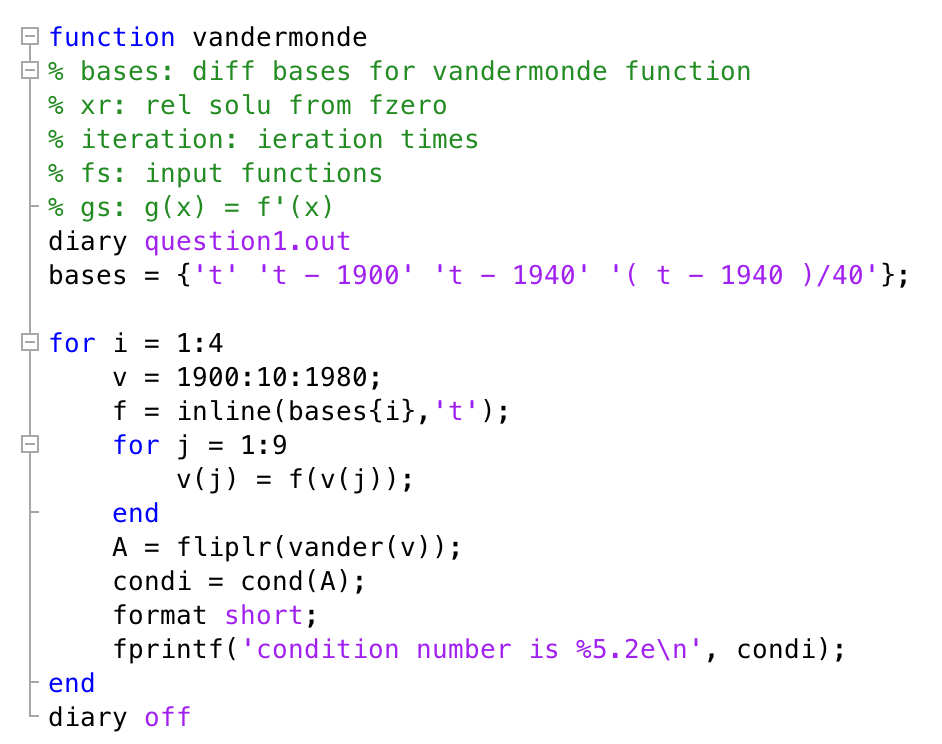
\includegraphics[scale=0.7]{1code} \]
	\[ 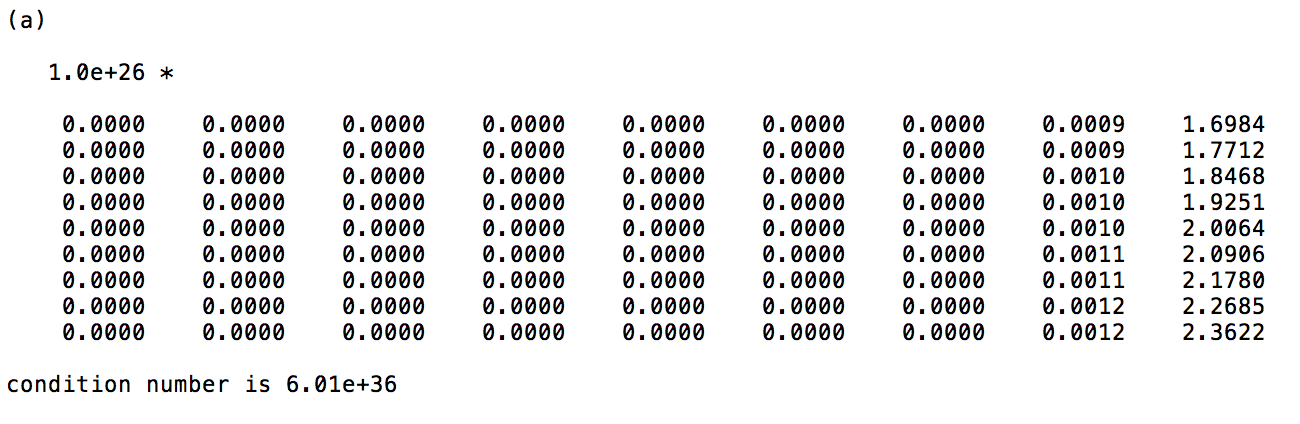
\includegraphics[scale=0.6]{1a} \]
	\[ 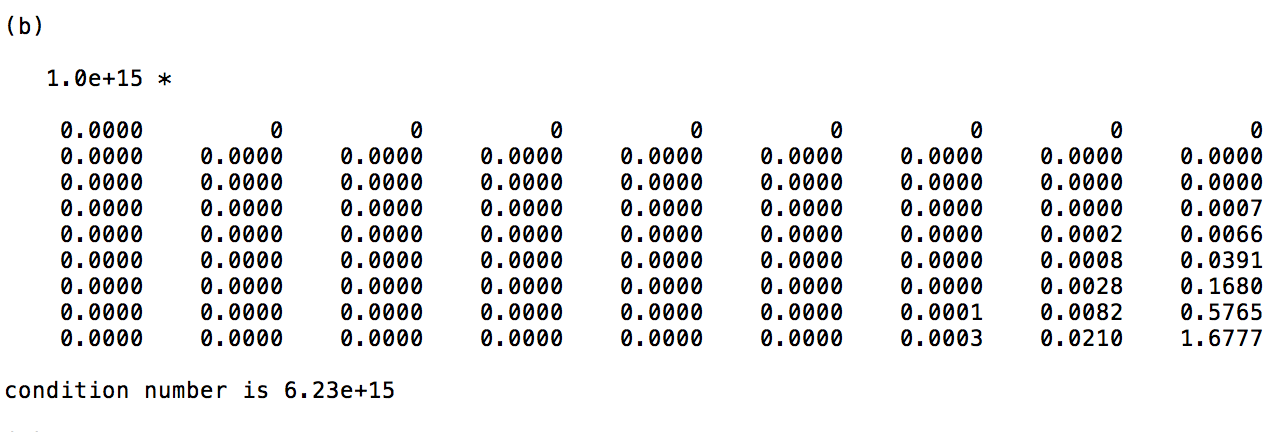
\includegraphics[scale=0.6]{1b} \]
	\[ 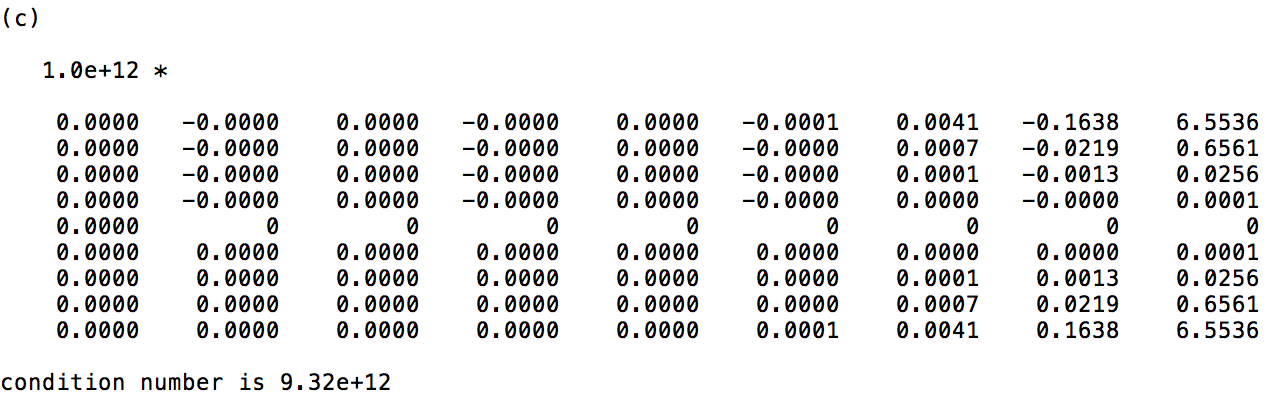
\includegraphics[scale=0.6]{1c} \]
	\[ 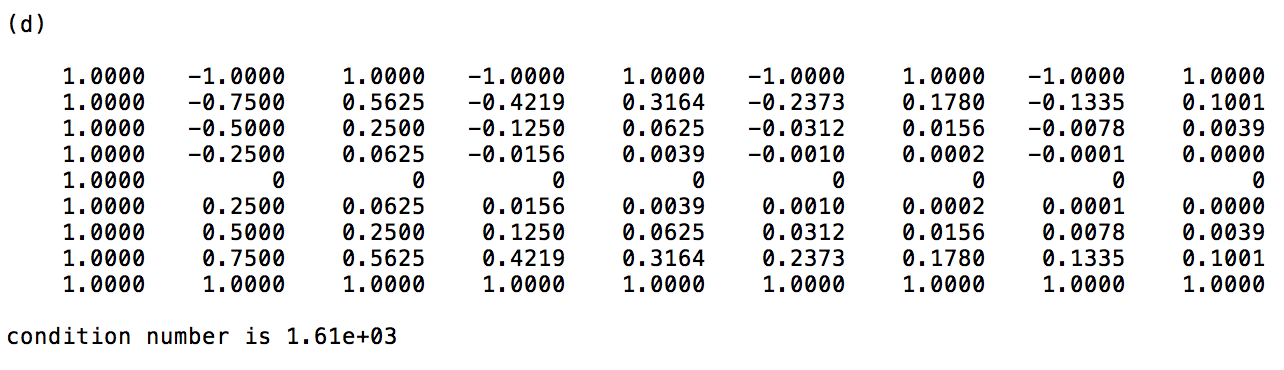
\includegraphics[scale=0.6]{1d} \]
\begin{itemize}	 
\item First we could notice that the condition numbers for $(a)$, $(b)$, $(c)$ are large and they are ill-condition. 
And the condition numbers are decreasing  from $(a)$ to $(d)$; hence, clearly we should recommend $(d)$.
\item Also, The functions are exponential functions with exponent bigger than $1$. Then they all grow rapidly for base number with  absolute value bigger than 1.
\item  for (a)  the base numbers are all bigger than 1900, 
which makes the function grows even faster. Therefore, comparing with last few columns, rest columns are too small, which make the Vandermonde matrix nearly singular. Same for $(b)$ base numbers are still big.
\item For $(c)$, $t-1940$ makes the base number symmetric about $1940$, but since the absolute value for most the of base numbers are still bigger than $10$, then it still grows fast as the exponent increases, which makes the Vandermonde matrix nearly singular.
\item For $(d)$, $\frac{(t-1940)}{40}$ makes all base numbers between $[-1, 1]$, then the value are changing relative slow compare with $(a)$, $(b)$ and $(c)$ which have bases number bigger than $10$.   
\end{itemize}
For all those reasons have been discussed above, I would recommend  the function $d$ to generate an interpolant if the Vandermonde approach is used. 
% question 2
\item \proc{solution}:
\begin{enumerate}
%part a
\item Using \textbf{matlab}'s \textbf{polyfit}$([-1,2,3,5], \ [0,1,1,2], \ 3)$, we get $[ \frac{1}{24}, \frac{-1}{4}, \frac{11}{24}, \frac{3}{4} ]$. \\
Hence, the function we get from polynomial interpolant using monomial basis is, 
\[\frac{1}{24}x^3 - \frac{1}{4}x^2 + \frac{11}{24}x + \frac{3}{4}\]
% part b
\item Using \textbf{Lagrange}  polynomial interpolant we get,
			\begin{align} \nonumber
                             \ P_3(x)  & = 0 + \frac{(t+1)(t-3)(t-5)}{(2+1)(2-3)(2-5)} + 
                             		\frac{(t+1)(t-2)(t-5)}{(3+1)(3-2)(3-5)} + \frac{2(t+1)(t-2)(t-3)}{(5+1)(5-2)(5-3)} \\ \nonumber
			   \ P_3(x)  & = 0 + \frac{t^3-7t^2+7t+15}{9} + \frac{t^3-6t^2+3t+10}{-8} + \frac{2t^3-8t^2+2t+12}{36} \\ \nonumber
			    \ P_3(x)  & =  \frac{8t^3-56t^2+56t+120}{72} + \frac{9t^3-54t^2+27t +90}{-72} +  \frac{4t^3-16t^2+4t+24}{72} \\ \nonumber
			     \ P_3(x)  & =  \frac{3t^3-18t^2+33t+54}{72} \\ \nonumber
			     \ P_3(x)  & = \frac{1}{24}x^3 - \frac{1}{4}x^2 + \frac{11}{24}x + \frac{3}{4} \nonumber
                        	\end{align}
Clearly, using \textbf{Lagrange}  polynomial interpolant we get the same polynomial with $(a)$.
%part c
\item  Using \textbf{Newton} polynomial interpolant (Divided Differences) we get,  
			\[x_0 = -1\hskip0.5pc  y_0 = 0 \hskip12pc  \]
						\[\hskip7pc  \frac{1}{3} \hskip5pc\]
			\[x_1 = 2\hskip1pc  y_1 = 1 \hskip7pc   \frac{-1}{12} \hskip4pc\]
						\[ \hskip9pc  \frac{0}{1}  \hskip6pc  \frac{1}{24}\]
			\[x_2 = \ 3\hskip1pc  y_2 = 1 \hskip7pc  \frac{1}{6} \hskip4pc\]
						\[\hskip7pc  \frac{1}{2} \hskip5pc\]
			\[x_3 = \ 5\hskip1pc  y_3 = 2 \hskip12pc \]
	Hence we have,
			\begin{align} \nonumber
			 \ P_3(x) &= \frac{1}{3}(x+1) - \frac{1}{12}(x+1)(x-2) +\frac{1}{24}(x+1)(x-2)(x-3) \\ \nonumber
			 \ P_3(x) &= \frac{1}{3}(x+1) - \frac{1}{12}(x^2 - x - 2) +\frac{1}{24}x^3 - 4x^2 + x + 6\\ \nonumber
			  \ P_3(x) &= \frac{1}{24}x^3 - \frac{1}{4}x^2 +\frac{11}{24}x +\frac{3}{4} \nonumber
			 \end{align}
Clearly, using \textbf{Lagrange}  polynomial interpolant we get the same polynomial with $(a)$.			
\end{enumerate}
% question 3

\item  \proc{solution}:
\begin{enumerate}
	\item \[ 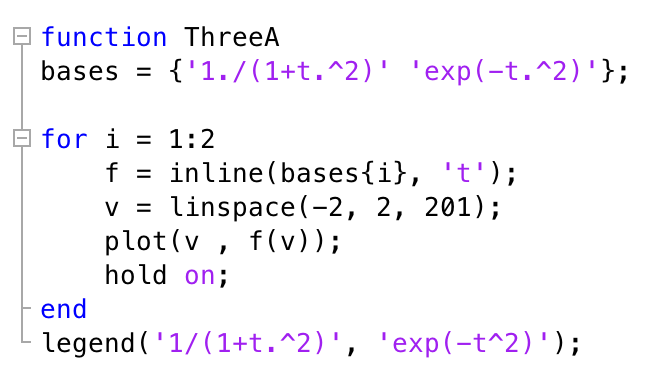
\includegraphics[scale=0.6]{code3a} \]
		\[ 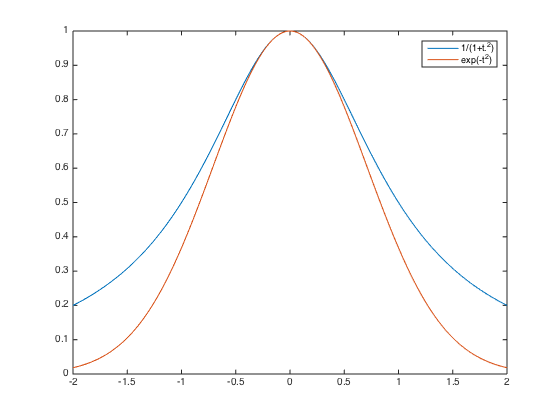
\includegraphics[scale=0.6]{3a} \]
	\item \[ 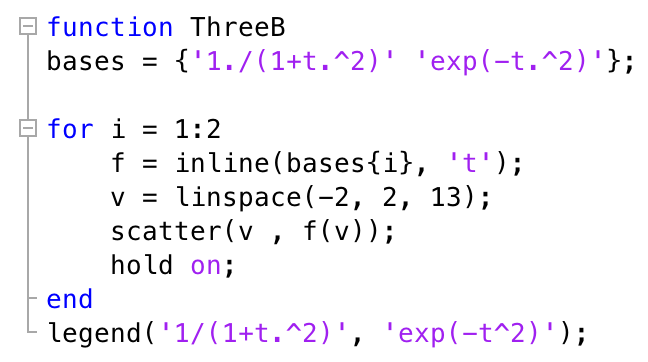
\includegraphics[scale=0.6]{code3b} \]
		 \[ 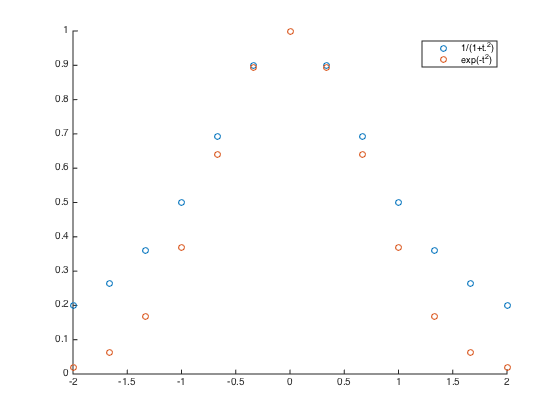
\includegraphics[scale=0.6]{3b} \]
		\[ 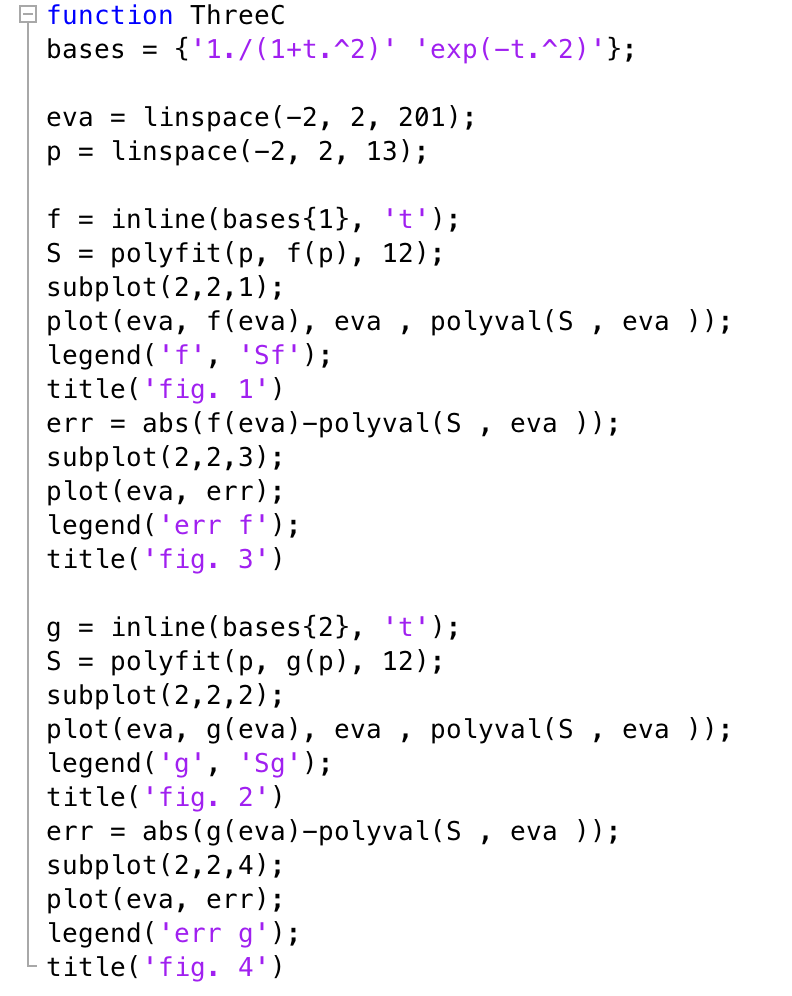
\includegraphics[scale=0.5]{code3c} \]
	\item \[ 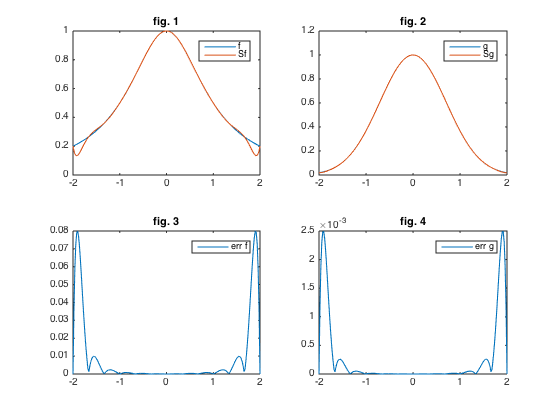
\includegraphics[scale=0.8]{3c} \]
	\item It is clear that $g(t) = \exp^(-t^2)$ has a better approximation compare with $f(t) = \frac{1}{1+t^2}$.
		And we could see, for $f(t) = \frac{1}{1+t^2}$ when $t$ is close to end points $2,-2$, the approximation become worse. This is because the lack of the uniformly convergence of the polynomial interpolants to an underlying continuous function as the number of equally spaced points increases.
	\item	 \[ 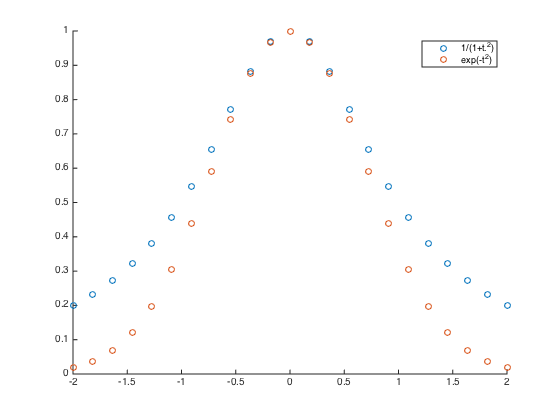
\includegraphics[scale=0.4]{3e1} \]
		 \[ 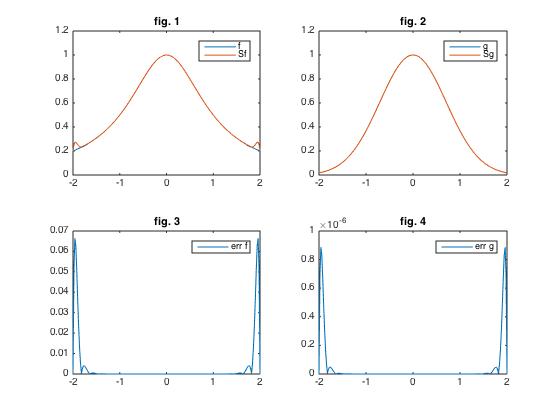
\includegraphics[scale=0.8]{3e2} \]
\end{enumerate}
% question 4
\item 
\proc{solution}:
\begin{itemize}[label = {}]
\item We know that for piecewise polynomial interpolation, the absolute error $e \leq \frac{max(\ f''(x) \ ) \ \cdot \ h^2}{8}$, where $x \in [0, \pi /2]$ and  $h$ is the length of the longest subinterval in the partition.
			\[max ( |f''(x) | )=max ( | \sin''(x) | )=max ( | sin(x) | ) = 1 \]
\item Since, the question asked for a absolute error within $1.0 \times 10^{-4}$, then we have,
					\begin{align} \nonumber
                                        		\ \frac{max(\ f''(x) \ ) \ \cdot \ h^2}{8} &  \leq 1.0 \times 10^{-4}  \\ \nonumber
						\ \frac{1 \ \cdot \ h^2}{8} &  \leq 1.0 \times 10^{-4}  \\ \nonumber
						\ h^2 			     &  \leq 8.0 \times 10^{-4}  \\ \nonumber
						\ (\frac{\pi}{2(n-1)} )^ 2&  \leq 8.0 \times 10^{-4}  \hskip1pc  n \ is \ the \ total \ number \ of \ enties\\ \nonumber
						\ \frac{\pi}{2(n-1)} 		     &\leq  \sqrt{ 8.0 \times 10^{-4}}  \\ \nonumber
						\ 2(n-1) 		     &\geq \frac{\pi} {\sqrt{ 8.0 \times 10^{-4}}}  \\ \nonumber
						\ n 		     &\geq \frac{\pi} {2\sqrt{ 8.0 \times 10^{-4}}} +1 \\ \nonumber
						\ n 		     &\geq 56.5360  \nonumber
                        			\end{align}
Hence, 57 entries are needed in order to make the absolute error within $1.0 \times 10^{-4}$.
\end{itemize}
% question 5
\item 
\begin{enumerate}
\item   \[ 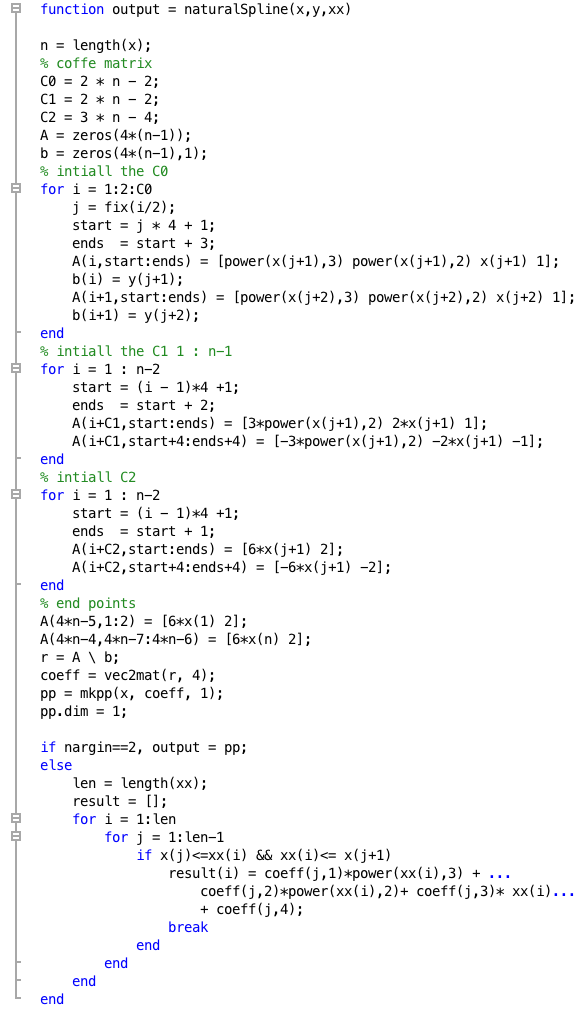
\includegraphics[scale=0.8]{code5b(i)} \]  
	We use $[(0 0),(1 ,1),(2, 8)]$ test we suppose to get, 
			\[ p_1(t) = a_1 x^3 + a_2 x^2+ a_ 3 x+ a_4\]
			\[ p_2(t) = b_1 x^3 + b_2 x^2+ b_ 3 x+ b_4\]
			\[ a_4 = 0\]
			\[a_1 + a_2 + a_ 3 + a_4 = 1 \]
			\[b_1 + b_2 + b_ 3 + b_4 = 1\]
			\[8b_1 + 4b_2 +4 b_ 3 + b_4 = 8\]
			\[3a_1 + 2a_2 + a_ 3  = 3b_1 + 2b_2 + b_ 3 \]
			\[6a_1 + 2a_3  = 6b_1 + 2b_2 \]
			\[ 2a_3  = 0 \]
			\[12b_1 + 2b_2 = 0 \]
	solve the eqaution we get,
			\[ p_1(t) = 1.5 x^3 -0.5x\]
			\[ p_2(t) = -1.5 x^3 + 9x^2-9.5x + 3 \]
	and the result from $naturalSpine$ is same with our calculation,\\
	matrix of coefficient:
	  \[ 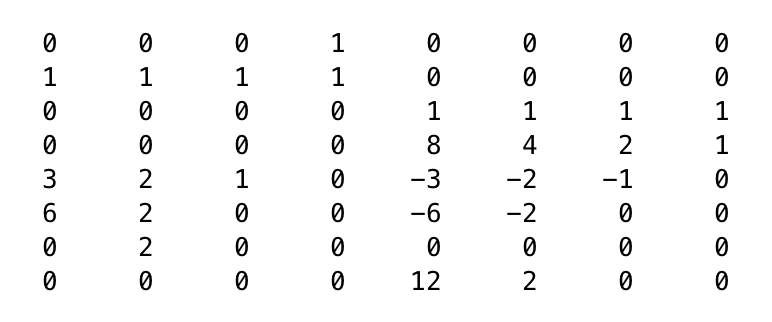
\includegraphics[scale=0.4]{m} \]  
	 coefficient:
	    \[ 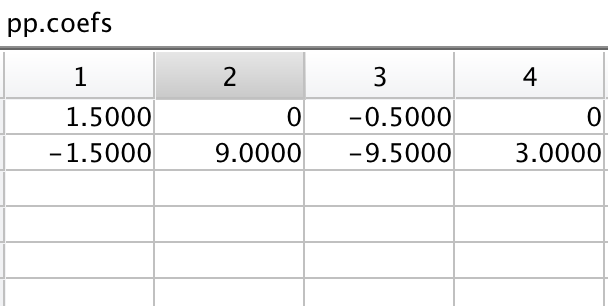
\includegraphics[scale=0.4]{r} \]  
\item 
	\begin{enumerate}
	\item The results we generate from sample $\{0,1,2,3,4,5\}$ are,
	  \[\{  0, \ \ 0.3679, \ \ 0.2707,   \ \  0.1494,  \ \   0.0733, \ \   0.0337\}\]
	\item   \[ 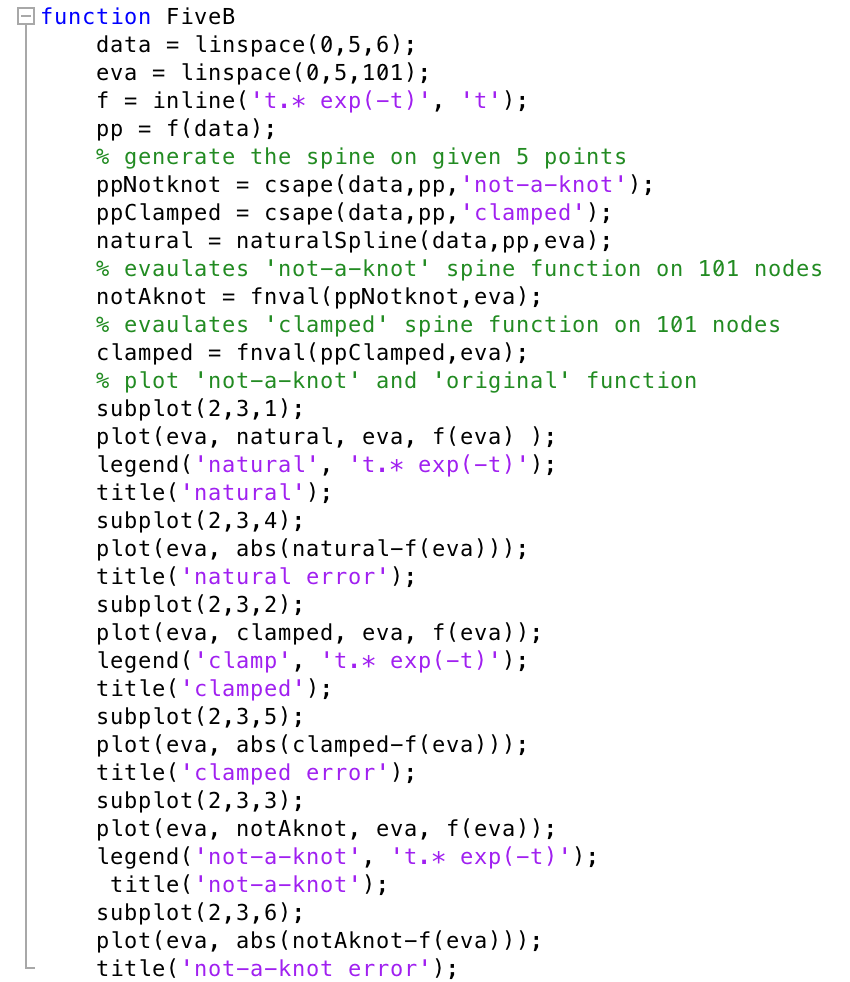
\includegraphics[scale=0.6]{code5b(ii)} \]
		  \[ 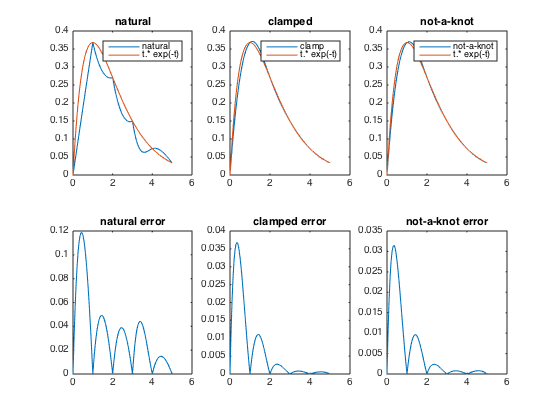
\includegraphics[scale=0.7]{5b(ii)} \]  
	\item 
		 \[ 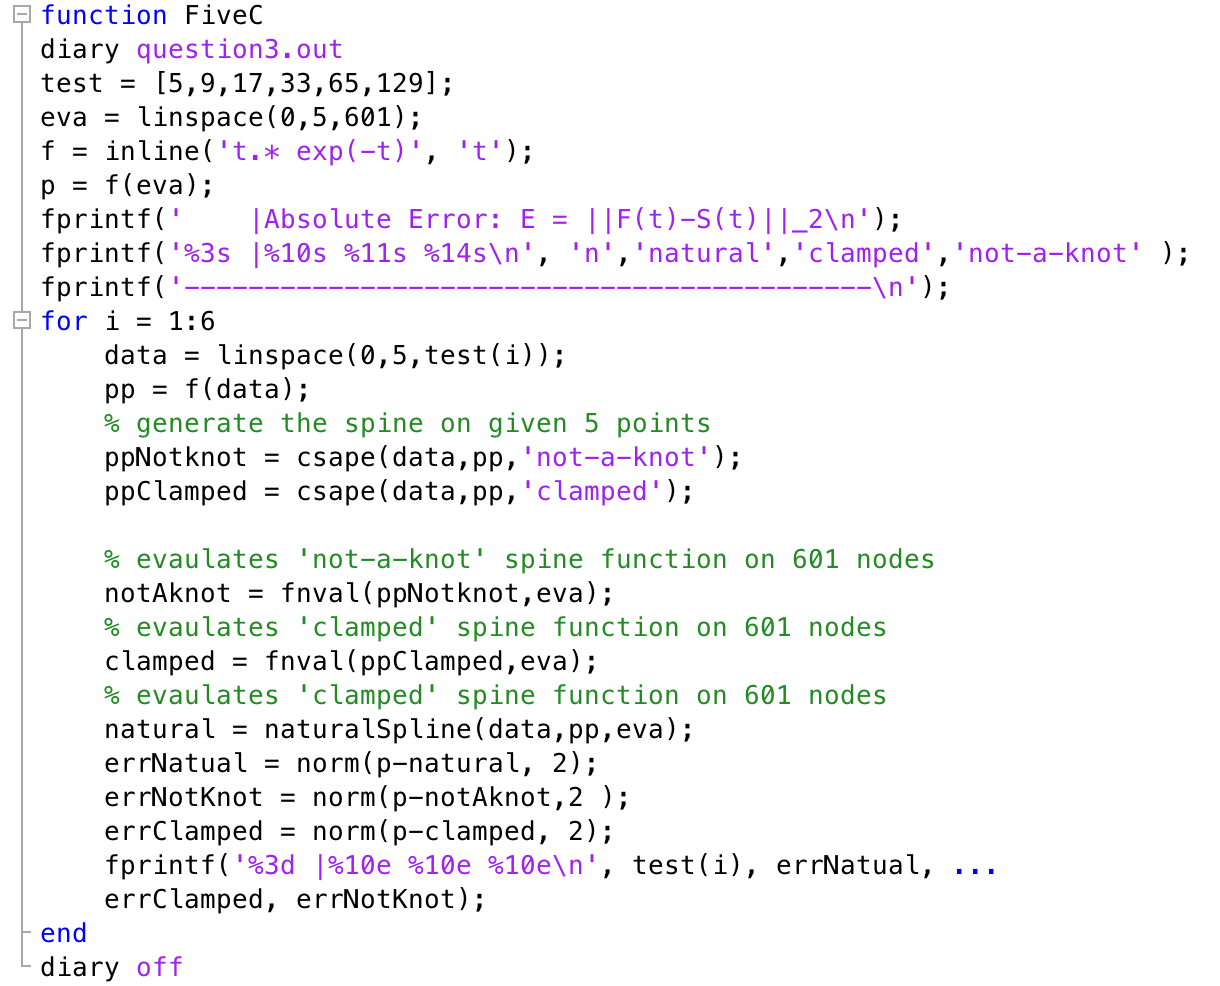
\includegraphics[scale=0.5]{code5b(iii)} \]  
		  \[ 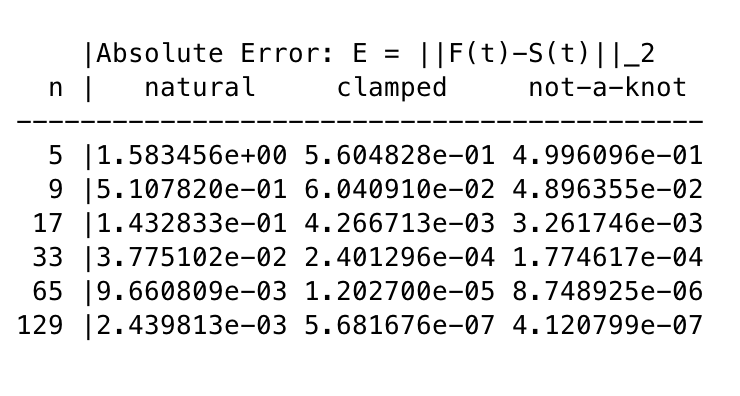
\includegraphics[scale=0.7]{5b(iii)} \]  
	\end{enumerate}
\end{enumerate}
\end{enumerate}

\end{document}